\documentclass{article}

% if you need to pass options to natbib, use, e.g.:
%     \PassOptionsToPackage{numbers, compress}{natbib}
% before loading neurips_2020

% ready for submission
\usepackage[final]{neurips_2020}

% to compile a preprint version, e.g., for submission to arXiv, add add the
% [preprint] option:
%     \usepackage[preprint]{neurips_2020}

% to compile a camera-ready version, add the [final] option, e.g.:
%     \usepackage[final]{neurips_2020}

% to avoid loading the natbib package, add option nonatbib:
% \usepackage[nonatbib]{neurips_2020}
\usepackage[utf8]{inputenc} % allow utf-8 input
\usepackage[english]{babel}
\usepackage[T1]{fontenc}    % use 8-bit T1 fonts
\usepackage[colorlinks = true, urlcolor = blue, citecolor = black, filecolor = black, linkcolor = black]{hyperref}       % hyperlinks
\usepackage{url}            % simple URL typesetting
\usepackage{booktabs}       % professional-quality tables
\usepackage{amsfonts}       % blackboard math symbols
\usepackage{nicefrac}       % compact symbols for 1/2, etc.
\usepackage{microtype}      % microtypography
\usepackage[
backend=biber,
style=numeric,
sorting=ynt
]{biblatex}

\usepackage{graphicx}
\usepackage{subcaption}
\addbibresource{ref.bib}


\title{Riiid! Answer Correctness Prediction}

% The \author macro works with any number of authors. There are two commands
% used to separate the names and addresses of multiple authors: \And and \AND.
%
% Using \And between authors leaves it to LaTeX to determine where to break the
% lines. Using \AND forces a line break at that point. So, if LaTeX puts 3 of 4
% authors names on the first line, and the last on the second line, try using
% \AND instead of \And before the third author name.

\author{%
  Tiago Antunes$^1$, Sahand Sabour$^1$, Henry Zheng$^1$  \\
  Department of Computer Science and Technology\\
  Tsinghua University, Beijing, China\\
  \texttt{\{vazama10,shanm20,zheng-jh20\}@mails.tsinghua.edu.cn}
}

\begin{document}

\maketitle

\begin{abstract}
    Knowledge Tracing is the process of modeling students' understanding of a knowledge concept based on their interactions with a series of exercises and learning activities. With the recent COVID-19 pandemic and rise of online education, the field of knowledge tracing is highly essential as it provides students with their own customized learning experience. In this project, we were tasked to employ a new knowledge tracing model and/or improve upon previous state-of-the-art work to accurately predict whether a student would answer a given exercise correctly, given his/her performance history. We implemented two commonly used transformer-based models using PyTorch. We further analyze the problem to understand what were our difficulties when dealing with the task, what were the steps we took and the results that were obtained.
\end{abstract}

\section{Introduction}

Due to the recent COVID-19 pandemic and rise of need for social distancing, numerous schools have been temporarily closed. Many organizations have transferred their events and activities to virtual environments. This has led the society to switch to online educational courses, material, and environments. As these platforms provide a significant amount of information for students' learning activities, attentiveness, and performance, they can provide valuable data for further analysis to improve on the online learning experience. Hence, the topic of Knowledge Tracing has become highly essential and has gained considerable attention from the research community. Knowledge tracing (KT) can be defined as the task of modeling students' comprehension regarding knowledge concepts (KCs) upon their interactions with a series of learning tasks, exercises, and coursework. Accordingly, an accurate KT model can be utilized to predict students' performance in future interactions, which was our goal during this project. Hence, knowledge tracing is crucial for providing students with personalized learning experiences, which allows them to choose subjects based on their needs and obtain relative knowledge with appropriate tasks and exercises.

In general, KT can be formalized as a supervised learning task, where given the exercise history $E= {e_1, e_2, ..., e_t}$ and the binary student response history $R = {r_1, r_2, ..., r_t}$ (with 1 representing a correct response), the aim is to predict the probability of the student submitting a correct response to the next exercise; i.e. $p(r_{t+1}=1|e_{t+1})$. Early approaches focused on deep learning for constructing KT models, with Deep Knowledge Tracing (DKT) \cite{Piech2015} and Recurrent Neural Networks (RNN) gaining more attention. Several approaches, such as Dynamic Key-Value Memory Networks (DKVMN) \cite{Zhang2017}, which utilized key and value matrices to model the relationship between students' knowledge level and the provided exercises, have also gained some attention, mainly due to their superior interpretability in comparison with prior deep learning models. Recent work has built upon the success of transformers \cite{Vaswani2017} and has produced state-of-the-art performance \cite{Choi2020}.

In this paper, we introduce two highly accurate, transformer-based Knowledge Tracing models that were utilized for this competition: Self-Attentive Knowledge Tracing (SAKT) \cite{Pandey2019} and Separated Self-Attentive Neural Knowledge Tracing with Temporal Features (SAINT+) \cite{Shin2020}. Accordingly, we demonstrate and explain our implementations of these models and the employed methodology. Lastly, we provide the obtained evaluation results of our implemented models based on the \emph{Riiid! Answer Correctness Prediction} dataset, which was provided for this competition on \emph{Kaggle}. 


\section{Related Work}

\subsection{Bayesian Knowledge Tracing}
The Bayesian Knowledge Tracing model initially proposed by Corbett \& Anderson \cite{Corbett1995} has been used in several parts of the industry, which introduces the \textit{learning parameters} and the \textit{mediating parameters} split \textbf{S}, the probability that although the student has the knowledge he might give a wrong answer, and guess \textbf{G}, the probability of guessing it right although the student has no knowledge on the topic, building the basis for Knowledge Tracing. Nevertheless, this model has a few problems \cite{Baker2008} regarding its parameters that can be solved as, for example, \textit{Model Degeneracy}.

\subsection{Deep Neural Network Knowledge Tracing}
Recently, deep neural networks have become the most popular tool to approach Knowledge Tracing \cite{Xiong2016} due to their higher performance upon the Bayesian Knowledge Model which is widely seen as the base for this problem. The usage of Recurrent Neural Networks (RNN) is due to them being able to represent knowledge over time, relating automatically to the temporal characteristic of the problem and being able to learn from data instead of being hand-tuned similarly to previous work on the area, giving origin to Deep Knowledge Tracing (DKT). It was also introduced the concept of Long Short-Term Memory (LSTM) which solves the vanishing gradient problem and also improved the performance of the RNN in the Knowledge Tracing problem over BKT and PFA. 

Improvements can still be made upon the given RNN with LSTM model taking into account the human factor of learning something. As stated in previous research \cite{Minn2018}, each person has a different learning ability and therefore need to be considered differently than other with a different learning ability (while also taking into account the past knowledge at a time). At the same time, knowledge that has been acquired recently is much more likely to still be remembered comparing to previous one \cite{Yang2020} and the short-term memory effect needs to be taken into account. For this, it was used Convolutional Neural Networks (CNN) which was able to include this detail into its model, ending up with Convolutional Knowledge Tracing (CKT) which, due to its convolutional nature, requires a change of the underlying data representation from one-hot encoding to a matrix format.

\subsection{Graph Neural Network Knowledge Tracing}
Graphical Knowledge Tracing (GKT) approach tackles the learning of high-order relation information between the knowledge and question\cite{Yang2020, Tong2020}, the long term dependencies of the questions \cite{Yang2020} and at the same time maintaining the interpret-ability of the model \cite{Nakagawa2019}. In KT scenarios, some questions may require understanding of multiple knowledge areas to answer a single question. Conversely, a single knowledge area may also be used to answer different kinds of questions. These predictive models assumes the students' mastery of knowledge means the students could answer the corresponding question correctly. However, this assumption neglects the idea that the level of difficulty may affect the accuracy to different questions answered by the student \cite{Yang2020}. GNN approach aggregates knowledge and question embedding to mitigate these issues. Including a attention mechanism to prevent loosing of long-term dependencies information as the model training goes further \cite{Yang2020}. Other than these benefits, GNN models can also provide better interpretable prediction results that BKT and DKT models \cite{Nakagawa2019}.

\subsection{Key-Value Memory networks}
One of the main problems of Bayesian-based approaches such as BKT \cite{Baker2008} is their lack of ability to establish the relationship between different knowledge concepts. In addition, deep models such as DKT \cite{Xiong2016} fail to track the level of comprehension for each individual knowledge concept as these models merely produce a single collective state for all KCs. Hence, in order to tackle the shortcomings of these two types of approaches, Dynamic Key-value Memory Networks (DKVMNs)\cite{Zhang2017} were introduced. In these networks, key and value matrix pairs are used to construct a more powerful memory than LSTMs in terms of storing the history of student performances. Accordingly, at each time stamp, input features or tags are written as immutable keys, the exercise-response tuple $(e_t, r_t)$ is written to or read from the value matrix, and the probability of a correct response $p(r_{t+1}=1|e_{t+1})$ is produced as output. Therefore, DVKVMs are able to overcome the barriers of both BKTs and DKTs by realizing the relationship between different KCs while providing the ability to track each KC individually.

\section{Methodology}

\subsection{Problem Definition}
The main objective of our DAKT model is to accurately predict students' performance on future exercises, given a history of their behavior on the \emph{Santa} platform. Essentially, for \emph{n} number of students' behavior history can be represented as an adjacency matrix $(R, F)^{n}$, where $F_i \in\mathbb{R}^{d}$ and $R_i \in \{0,1\}$. $F_{i}$ is a feature vector for the given entries in the dataset, and $R_{i}$ is the corresponding user answer; Hence, the problem can be formulated as correctly predicting the following probability
\begin{center}
    $P(R_{i}=1|F_{i})$
\end{center}
where $F_{i}$ is the current question that the user needs to guess.

\subsection{Input Representation}
\label{input_representation}
Our model accepts the \emph{Riiid! Answer Correctness Prediction} dataset, which is provided on \emph{Kaggle}, as input. This dataset is in a question-response sequence format. Its major property is that the questions are collected in bundles; that is, questions regarding a common topic are provided as a collective bundle. In addition, for this competition, the given dataset is divided into three parts: train data, questions, and lectures.

As the name suggests, the train data is the essential part of training the model and it contains the following attributes:
\begin{itemize}
    \item Row ID: A unique ID for each entry in the dataset.
    \item Timestamp: The duration between the user's first event completion and this interaction.
    \item User ID: A unique ID for the student who is responsible for this interaction.
    \item Content ID: A unique ID for the interaction corresponding to this entry.
    \item Content Type ID: Shows whether the relative interaction was a question or a lecture.
    \item Task Container ID: Represents the bundle for this interaction.
    \item User Answer: The answer provided by the student.
    \item Answered Correctly: Shows whether the provided answer is correct.
    \item Prior Question Elapsed Time: The average time (in milliseconds) that it took the student to complete the prior bundle.
    \item Prior Question Had Explanation: Shows whether the student was provided with an answer or an explanation upon completing the previous bundle.
\end{itemize}

The lectures and questions portion of the dataset are utilized to provide more information regarding a specific interaction, based on the mentioned \emph{Content ID}. These portions include the following attributes:
\begin{itemize}
    \item ID: A foreign key for the Content ID in the train data portion.
    \item Bundle ID: A unique ID for the corresponding bundle (only available for questions).
    \item Correct Answer: The correct answer for the given interaction (only available for questions).
    \item Part: Top level category for this interaction based on the sections of the TOEIC test.
    \item Tags: Detailed tag codes for the given interaction. Questions have one or more tags while lectures can only have one tag.
    \item Type: a brief description of the purpose of this interaction (only available for lectures).
\end{itemize}

\subsection{Dataset Insights}
\label{data_insights}
Based on initial exploratory data analysis on the provided dataset, we found several interesting relationships between the features:
\begin{itemize}
    \item There are a total of 393656 students, from which around 4\% have answered more than 1500 questions. They are not representative of the whole dataset. 60\% of the users answered only up to 61 questions.
    \item Most of the users use the system for a short period of time and drop out after
    \item One third of the questions are answered incorrectly
    \item If the prior question had explanation, the students have higher tendency of getting the answer correctly.
    \item The percentage of answered questions increases with the number of questions answered, but there are many outliers (\textbf{This doesn't include same tag questions only})
    \item There's no need to be careful with lectures and questions mixed in the same task container as they all have the same timestamp. It's possible to assume previous and post questions times, which makes it simpler.
    \item Students get more correct answers on some specific tags, since the number of answers per tag also matters.
\end{itemize}

 
\subsection{Attention-based Knowledge Tracing}
The models implemented for this Kaggle competition are Self-Attentive Knowledge Tracing (SAKT)\cite{Pandey2019} and SAINT+\cite{Choi2020, Shin2020}. SAKT and SAINT+ model has similar architecture, and both are created based on the transformer model \cite{Vaswani2017}.

\begin{figure}[h]
\begin{subfigure}{.5\textwidth}
  \centering
  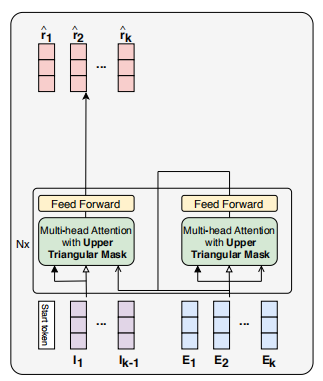
\includegraphics[width=.8\linewidth]{SAKT.png}
  \caption{SAKT}
  \label{fig:SAKt}
\end{subfigure}%
\begin{subfigure}{.5\textwidth}
  \centering
  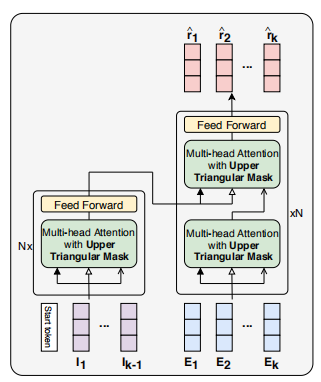
\includegraphics[width=.8\linewidth]{SAINT.png}
  \caption{SAINT}
  \label{fig:SAINT}
\end{subfigure}
\caption{Implemented model architectures \cite{Choi2020}}
\label{fig:fig}
\end{figure}

Transformers use attention-mechanism for transforming a sequence of input into another sequence by using encoders and decoder in the architecture. Encoder and decoder in transformers are composed of stacked of multiple Multi-Headed Attention network and Feed Forward Networks (FFN). During training, the input sequences and targeted sequences are transformed into embedding representations of size $S$ for input sequence and size $T$ for target sequence where $S$ is the number of the features of each entry in input sequences and $T$ is the number of features of each entry in the output sequences. In our case, an input sequence is a sequence of questions given to a specific user plus the meta data of the characteristics of him/her answering the question. Then an output sequence is a sequence of the correctness of his/her response to the questions. Then input sequence embedding and target sequence embedding are fed into the encoder and decoder respectively. 

The Multi-Headed Attention networks of the transformers are multiple attention networks that are applied multiple times to the same input sequence with difference weights. The attention network takes inputs $Q_{in}$, $K_{in}$, and $V_{in}$ \cite{Choi2020}. In our implementation, $Q_{in}$ is a matrix that consist of stacked queries, which are vector representations of an single question and its meta data of a user; $K_{in}$ is a matrix that consist of staked keys, which are vector representations of the questions done and their meta data the by the users; and finally, $V_{in}$ is a matrix of the values, which are vector representations of the correctness of the responses of the user to the questions. The attention network projects the $Q_{in}$, $K_{in}$, and $V_{in}$ to latent space by multiplying with learned weights $W^Q$, $W^K$, and $W^V$ then yields $Q$, $K$, and $V$ respectively. In calculation of attention weights, a upper triangular mask was applied to the matrix $QK^T$ to prevent the model to attend to the future features in the sequence. This is done by setting $-\infty$ to the values to be hidden then applying a softmax operation. Then the attention network head, $head_i$, is by multiplying the attention weights to the $V_i$, as shown as follows, $$head_i = Softmax(Mask(\frac{Q_iK_i^T}{\sqrt{d}}))V_i$$
Then a Multi-Headed Attention Network is a concatenation of h attention heads multiplied by learned weight $W^O$ as denoted by, $$MultiHead(Q_{in}, K_{in}, V_{in})=Concat(head_1,...,head_h)W^O$$

Both the encoder and the decoder blocks include a Feed Forward Network (FFN) which occurs after the multi-headed attention layer. This is a very thin layer that simply does $$FFN(x) = ReLU(xW_1 + b_1)W_2 + b_2$$ where $W_1, W_2$ are the weights and $b_1, b_2$ are biases. \cite{Choi2020}

The SAKT and SAINT models have similar transformer network architecture. Their only difference in our implementations are the features and embedding used and the number of Multi-Headed Attention layers in encoder and decoder modules.
\subsection{Input Preprocessing}
\label{input_preprocessing}
The dataset used in the competition was \emph{Riiid! Answer Correctness Prediction}, which has been described in detail in \autoref{input_representation}. In order to have an efficient model, pre-processing of the provided data is highly necessary as it allows us to extract and highlight the important features. It also enables us to remove unwanted features (i.e. noise) that could severely harm the model.

We transformed the dataset from a per-row interaction into a user-data format. To this end, we grouped all user data into a single object for ease of access. This allows for increased data locality and speed when looking for the user's past interactions. When doing this transformation, we also limited the number of user interactions to at a maximum of the last $windowsize$ elements. As stated in \autoref{data_insights}, many users replied to a low amount of questions. This means that given a sufficiently large $windowsize$, many users would stop having an enough amount of interactions, thus requiring us to \textit{pad} the data as to guarantee that the data server had the same length. This also included generating a mask for informing the models of what was padded or not.

In SAINT+ \cite{Shin2020}, a number of embeddings are used, which are mostly derived from the input data. However, one of implemented embeddings (\textit{lagtime}), which refers to the time between the submission of the previous exercise and the start of the current exercise, does not exist as an attribute of the dataset and must be calculated individually. Our calculation was as follows: given the timestamp of a new interaction $T_i$ and the timestamp of the previous user interaction $T_{i-1}$ we can then set the \textit{lagtime} of our new interaction $L_i$ as $$L_i = \min ((T_i - T_{i-1}) / 1000, 300)$$ thus getting the \textit{lagtime} in terms of seconds as a value between $[0, 300]$.
 
The dataset also provided meta-data about lectures and questions. We found it challenging to include the lectures in our models. Moreover, the addition of lecture did not seem to have a major impact on the obtained results. Hence, we simply ignored these interactions. With respect to the questions, we extracted the information relative to the \textit{part} of each questions and then assigned this part to each interaction by using a dictionary with $(question\_id, part)$ pairs as a way of efficiently mapping the relationship.

In summary, our processed data contains the following attributes:
\begin{enumerate}
    \item \textit{user\_id}
    \item a collection of queues with elements:
    \begin{itemize}
        \item \textit{content\_id}
        \item \textit{is\_correct}
        \item \textit{task\_container\_id}
        \item \textit{lagtime}
        \item \textit{prior\_question\_elapsed\_time}
        \item \textit{part\_id}
        \item \textit{padding\_mask}
    \end{itemize}
\end{enumerate}

When doing the inference, to improve the accuracy of the model, we would keep the information from before loaded in memory and use it to fetch the past user interactions. We would then update it, by removing the oldest interaction and adding the new one with the corresponding information, thus maintaining the $windowsize$ of the data.

\section{Results and Discussion}
Upon successful submission of our implemented models' predictions to Kaggle, our obtained Area Under Curve (AUC) scores were calculated and are provided respectively in the table below. 

For SAINT+ we used a number of layers, window size, model dimension, dropout and batch size of, respectively, 4, 100, 512, 0, 64. For SAKT we used window size and dropout of 128 and 0.2, respectively.

\begin{table}[h]
    \centering
    \begin{tabular}{|r|c|c|}
    \hline
        Model & Public score & Private score \\
        \hline
        SAINT+ (3 epochs) & 0.626 & 0.606 \\
        \hline
        SAINT+ (20 epochs) & 0.592 & 0.604\\
        \hline
        SAINT+ (encoder only) & 0.681 & 0.683\\
        \hline
        SAKT & \textbf{0.774} & \textbf{0.773}\\
        \hline
    \end{tabular}
    \vspace{0.2cm}
    \caption{Competition Results}
    \label{tab:results}
\end{table}

The model that performed the best was SAKT with a big difference from SAINT+. We believe this is due to an error in our SAINT+ implementation and also due to overfitting. 

Both our SAINT+ and SAKT implementations are not using the padding mask, as it was mentioned in \autoref{input_preprocessing}. Because we used PyTorch as the framework to build our model, in the end we stumbled upon an \href{https://github.com/pytorch/pytorch/issues/41508}{open issue} on the \textit{MultiHeadAttention} module which resulted in our results coming back as $NaN$. This further influenced our approach to use the padding mask, which reduced the accuracy of the model.

Another thing to be mentioned was that our SAKT model used a \textit{Feed Forward Network} in the end of its output before applying a linear transformation to output the result. Our SAINT+ is using an encoder-decoder paradigm (in which both encoder and decoder have a Feed Forward Network within them) and in the end is followed by a linear transformation. We believe that if before this linear transformation we included a Feed Forward Network we might be able to preserve more non-linear relationships, thus improving the result of the SAINT+ model, which is different from the original paper itself. We base this idea after analyzing a \href{https://www.kaggle.com/m10515009/saint-is-all-you-need-training-private-0-801}{public notebook from the competition} which is very similar to our approach with the exception  of that detail.

Another thing to be noticed from \autoref{tab:results} is our encoder only SAINT+. We initially submitted an incomplete version of SAINT+ that did not have a decoder. It consisted of just a few encoder blocks stacked on each other followed by a linear transformation. It also missed some extra details such as the \textit{lagtime} embeddings and the attention mask in comparison to the actual SAINT+ model. This model scored higher than our final model, from which we can derive two conclusions:
\begin{itemize}
    \item Data is noisy and the extra embeddings we used were not correctly calculated. On the previously mentioned public notebook, the author split the \textit{lagtime} into multiple \textit{lagtimes}, which correspond to seconds, minutes, and days respectively. We believe that this is a beneficial implementation for our future work.
    \item Following papers to implement their proposed models may not a good idea. We should work on establishing baselines to the given problem and try to improve them instead of directly implementing a paper without realizing it might not produce similar results in the given dataset.
\end{itemize}

\section{Conclusion}
To conclude, we analyze the project from the point of view of beginners to the field of Machine Learning. We see this competition as a great first experience working on a big project where we were able to apply much of the knowledge we learned during the semester. We believe it greatly contributed for us to improve our model building and paper reproduction skills and understanding more about the current area of ML. This competition allowed us to understand more how temporal relationships are built and we believe this new knowledge to be very valuable. In the future, we hope to build upon our lessons learned and achieve higher rankings in similar competitions.

\small
\printbibliography


\end{document}
